\subsection{Инициация поставки в хранилище}

\textbf{Участники:}
Менеджер, Администратор, Поставщик.

\textbf{Описание:}
Менеджер договаривается с Поставщиком о
поставке предметов в хранилище. Далее Менеджер 
создает в Системе заявку на поставку предметов в 
хранилище А. Администратор хранилища либо подтверждает 
заявку на поставку предметов, либо отклоняет ее. В 
любом процесс прекращается уведомлением Менеджера и 
поставщика.

\begin{figure}[h]
  \centering
  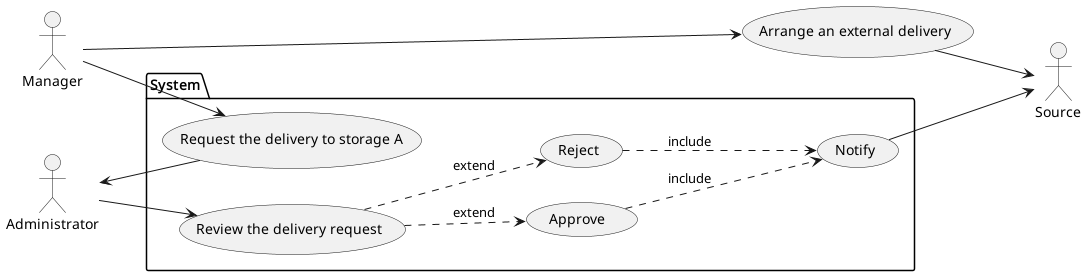
\includegraphics[width=12cm]{../../doc/spec/figure/usecase/delivery_arrange/Storage Net, Use Case, Delivery Arrange.png}
  \caption{Use Case: Delivery Arrange}
\end{figure}


\subsection{Принятие поставки предметов в хранилище}

\textbf{Участники:}
Администратор.

\textbf{Описание:}
Админимтратор ожидает прибытия предметов, после 
чего подтвержает прибытие предметов в хранилище.

\begin{figure}[h]
  \centering
  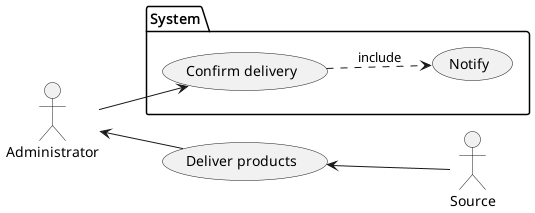
\includegraphics[width=12cm]{../../doc/spec/figure/usecase/delivery_confirm/Storage Net, Use Case, Delivery Confirm.png}
  \caption{Use Case: Delivery Confirm}
\end{figure}
